\chapter{Power Systems Background}

\label{ch:background}

\section{Structure and Organization of Power Systems}


  It is important to note that some power system studies are dependent on which power system is being studied; other studies pursue a more general understanding of power systems as a whole.  In this section we'll discuss characteristics of power systems, with a focus on the United States power system; however, most of these concepts are universal to all power systems throughout the world.

There is one rule that allows a power system to function: power generation and power demand must be instantaneously and continuously balanced.  This fact, while simple and concise, is difficult to achieve in practice.  Many of the rules and regulations surrounding power systems are to ensure that balance is maintained, or what procedures to follow should an imbalance occur.  In general, power systems are divided into transmission systems and distribution systems.  The regulations and procedures in part determine the physical structure of a power system, but it is also dependent on engineering choices and how power systems grew historically in a country.  In general, there are two main components of a power system: the distribution system and the transmission system.  Distribution systems tend to be tree-like network structures that deliver power to homes and commercial buildings.  Transmission systems are highly interconnected networks that exchange power between large regions.  The purpose of having a large system is that it makes it easier to balance power across multiple areas.  Due to the large areas that transmission systems cover, it is more efficient to use AC power, which allows for larger amounts of power for the same voltage level in DC power.  However, for safety reasons, distribution systems usually use DC power.  The mathematical distinction between AC and DC power will be discussed in Section \ref{ps:power}.  

\section{Power System Equations}
\label{ps:power}

A fundamental part of any power system study is a definition of how power flows from the sources to the sinks in the system.  These are referred to as the power flow equations (PFE), and they describe the the output power of every generator (sources) and the power flow on every line given the consumption of power at every bus.  For simplicity in our derivation, we assume that the power system we are modeling does not contain any capacitative effects, nor does it contain any transformers.  In particular, assuming zero capacitive effects means that current is conserved across the lines, and simplifies the power flow equations.  The derivation we present here is adapted from \cite{Bienstock2015}.  (ending sentence here)

\subsection{Power Flow Equations}
\label{sec:pfe}
First, we begin with some notation to represent the various components in the system.  A power system is represented by a set of buses (or nodes) and lines (edges).  Let the set of all buses in the system be represented by $N$ where $|N| = n_b$.  In a power system, buses can be generators, loads, or intermediaries.  Let the set of generator nodes be represented by $G$, where $|G| = n_g$ and the set of load nodes by $L$ where $|L|=n_l$.  Note that $G$ and $L$ are subsets of $N$, and a bus in $G$ can also be in $L$.  Intermediary buses are buses that do not consume or produce power, but instead help transmit power from the sources to the sinks.  Intermediary buses are all buses that are not in $G$ or $L$.  Finally, when we refer to lines in the system, we will denote this with a subscript of $ij$, which indicates the line that connects bus $i$ to bus $j$.

To begin our derivation, we start by defining the \textit{impedance},
\begin{equation}
\label{eqtn:impedance}
z_{ij}^* = r_{ij}+jx_{ij},\ \ \ i,j \in N	
\end{equation}
 where the real part $r_{ij}$ is the resistance of the line, and the imaginary part $x_{ij}$ is the reactance of the line.  Impedance describes the opposing force of the line to the alternating current (AC) power.  It quantifies how difficult it is for power to flow through the line.  Often, lines are instead quantified by their \textit{admittance},
\begin{equation}
\label{eqtn:admmitance}
y_{ij} = \frac{1}{z_{ij}} = g_{ij} + jb_{ij}	,\ \ \ i,j \in N	
\end{equation}
where $g_{ij}$ is the conductance, and $b_{ij}$ is the susceptance of the line.  Using Ohm's law, we can describe the complex current injected into a line by Equation \ref{eqtn:ohms}
\begin{equation}
\label{eqtn:ohms}
I_{ij} = y_{ij} (V_i-V_j)	,\ \ \ i,j \in N
\end{equation}

where $I$ is the current and $V$ is the voltage.  To write the complex power equation across a line, we introduce $\theta_i$ as the voltage angle at bus $i$, and $\theta_{ij} = \theta_i - \theta_j$.  Power is equal to the current times the voltage of a component, so the complex power across line $ij$ is
\begin{equation}
	\label{eqtn:complex_power}
	S_{ij} = V_iI^*_{ij} = y^*_{ij} |V_i|e^{j\theta_i}(|V_i|e^{-j\theta_i}-|V_j|e^{-j\theta_j})
\end{equation}

Often, power flow equations are expressed in polar coordinates, and complex power can then be separated into a real and imaginary part.  The real component represents the active power (denoted as $P$), and the imaginary part is the reactive power (denoted as $Q$).  Physically speaking, active power is consumed by resistive components (like your phone charger), and reactive power is consumed by reactive components (like your air conditioner).  Then, the real and reactive power across a line are defined by

\begin{subequations}
\label{eqtn:pf_line}
\begin{equation}
  P_{ij} = |V_i|^2 g_{ij} - |V_i| |V_j| g_{ij} \cos(\theta_{ij})-|V_i| |V_j| b_{ij}\sin(\theta_{ij})
    \label{eqtn:pf_l1}
\end{equation}    
\begin{equation}
 Q_{ij} = -|V_i|^2 b_{ij} +|V_i||V_j| b_{ij} \cos(\theta_{ij})-|V_i||V_j|g_{ij}\sin(\theta_{ij})
 \label{eqtn:pf_l2}
\end{equation}
\end{subequations}

Using Kirchoff's law, the real and reactive power at a node is defined as the sum of the real and reactive power of the lines connected to the node.

\begin{subequations}
\label{eqtn:pf_node}
\begin{equation}
  P_{i} = \sum_{j=1}^N P_{ij}
    \label{eqtn:pf_n1}
\end{equation}    
\begin{equation}
 Q_{i} = \sum_{j=1}^N Q_{ij}
 \label{eqtn:pf_n2}
\end{equation}
\end{subequations}


Equations \ref{eqtn:pf_l1} - \ref{eqtn:pf_n2} describe the AC power flow equations (ACPFE) in their entirety.  However, it is extremely common to linearize these equations, this is known as the DC approximation.  For this approximation, the following assumptions are made:

\begin{itemize}
	\item  $|V_i| \approx 1,\ \ \ \forall i \in N$
	\item $|\theta_{ij}|$ is small such that $\sin(\theta_{ij})\approx \theta_{ij}$
	\item For every line, the resistance is much smaller than the reactance, which means $g_{ij} \approx 0$ and $b_{ij} \approx \frac{-1}{x_{ij}}$
\end{itemize}
Using all of these assumptions, the real power flow across a line becomes $P_{ij} = -b_{ij} \theta_{ij}$.  Lastly, in the DC approximation we assume the reactive power consumption and production is constant.  This, along with the assumptions above, is generally what is meant by ``DC approximation" in cascading failure literature in  particular.

To solve the system of nonlinear equations a few parameters need to be given \textit{a priori}.  Usually, the real power ($P_i=P_{g}$), and voltage magnitude ($|V_i| = |V_{g}|$) of each generator is given, which is why they are often referred to as ``PV nodes" \cite{ferc_acopf}.  Every load node usually has its real power ($P_i = -P_{l}$) and reactive power ($Q_i = -Q_{l}$) specified, which is why they are often referred to as ``PQ nodes"\footnote{Note that the negative here means that real and reactive power are consumed at these nodes}.  Finally a reference node, often called the ``slack" node, is defined for the system and its voltage angle is set to zero ($\theta_i = 0$) and is used as a reference angle for every other bus in the system.  This node is required because we cannot know all power outputs prior to solving the equations because it depends on the steady-state of the system \cite{Takashi2015}.  Generally, the slack node is chosen to be the largest generator in the system because it will usually have sufficient real power to compensate for any deficits~\cite{ferc_acopf}.

It is extremely common to only use the power flow equations to study cascading failures for multiple reasons.  A large reason is that the addition of other dynamics increases the computational complexity, which can be prohibitive when studying a large number of outage scenarios.  However, it is becoming more common to also include generator dynamics when considering cascading failures, because it impacts the stability of the system, and as we will see in Chapter \ref{ch:cf}, it can change the severity of a cascade.  This next section outlines the necessary equations for modeling generator dynamics.
\subsection{Generator Dynamics}
\label{sec:gen_dyn}

Generators in power systems are usually described as phase oscillators, and often differences in power system stability studies differ by how loads are represented (\textit{i.e.} whether they are modeled as oscillators or not, and what kind)~\cite{Takashi2015}.  Here, we describe the \textit{structure preserving} model, which models load nodes as oscillators, or in other words, the consumption of power at load nodes is dependent upon the frequency of the generators.  Regardless of the model being used, all generator dynamics are derived based on Equation \ref{eqtn:swing} which defines the fundamental equation of motion for a generator, and is referred to as the \textit{swing equation} in the literature.
\begin{equation}
\label{eqtn:swing}
M_g\dot{\omega}_g + D_g\omega_g= P_{m_g} - P_{e_g},
\end{equation}
\begin{equation*}
\dot{\delta}_g = \omega_g -\omega_R, \ \ \ \forall g \in G
\end{equation*}


$M_g$ and $D_g$ are the inertia and damping constants of the generator, and are based on the type and mechanical specifications of the generator.  The inertia parameter $M_g$ can also be rewritten such that it has units of seconds, and can be directly related to the kinetic energy stored in the rotor of the generator
\begin{equation}
M_g \omega_r\pi = S_gH_g = KE_g
\label{eqtn:inertia}	
\end{equation}

where $S_g$ is the rated power of the generator.
The rotor angle, $\delta_g$, and frequency, $\omega_g$, of the generator are defined with respect to a rotating reference frame with a frequency of $\omega_R$ (60 Hz in the U.S. and 50 Hz in Europe). $P_{m_g}$ is the mechanical power input to the machine's rotor, and $P_{e_g}$ is the electric power demanded by the rest of the system.  For the structure preserving model and using the DC approximation assumptions, the equation of motion for generators is represented as a second order Kuramoto oscillator \cite{Dorfler}.


\begin{equation}
\label{eqtn:sp_gen}
	\dot{\omega}_g = -\frac{D_g}{M_g}\omega_g-\frac{1}{M_g}(P_g + \sum_{\forall i \notin G} b_{gi}\sin\delta_{gi}),\ \ \ \ \forall g \in G
\end{equation}

The load nodes (and all non-generator nodes, assuming they all have a frequency dependence) is then modeled by Equation \ref{eqtn:load}
\begin{equation}
\label{eqtn:load}
\dot{\delta_i} = -\frac{1}{D_i}(P_i + \sum_{\forall j \in N} b_{ij} \sin \delta_{ij}),\ \ \ \ \  \forall i \notin G
\end{equation}

where $D_i$ is the damping term that describes the frequency dependence of the node.  


More detailed descriptions of generator dynamics include the governor, which is responsible for controlling the generator frequency, and the excitation system, which controls the internal voltage magnitude of the generator.  However, the majority of cascading failure models discussed in Chapter \ref{ch:cf} do not consider these systems, and we will explicitly note when they do, so we will not discuss their equations here, and instead point the reader to the publications.


%\subsection{Power System Controls}
%Here is a section where I will just briefly mention the power system controls that most cascading failure studies implement.  The first and biggest is a limit on the amount of power that can flow on a line.  This is usually related to the thermal limit of the line (i.e. if the line gets too hot, it will ruin it).
%%%%%%%%%%%%%%%%%%%%%%%%%%%%%%%%%%%%%%%%%%%%%%%%%%%%%%
%%%%%%%%%%%%%%%%%%%%%%%%%%%%%%%%%%%%%%%%%%%%%%%%%%%%%%
%%%%%%%%%%%%%%%%%%%%%%%%%%%%%%%%%%%%%%%%%%%%%%%%%%%%%%
%%%%%%%%%%%%%%%%%%%%%%%%%%%%%%%%%%%%%%%%%%%%%%%%%%%%%%
\section{Understanding Power System Performance and Health}
%%%
\label{rel_stab_sec}
In North America, utility companies provide different system analyses to a variety of organizations.  This organizational structure is intended to promote safe and reliable flow across North America as more systems became connected to each other after growing independently with various operating conditions.  The intent of federal regulation is to create a uniform expectation across all power systems that hopefully makes it easier to have these systems interact with one another.  If power systems are not properly connected, failures can propagate throughout the system and cause severe damage, resulting in high financial costs.

\begin{figure}
\centering
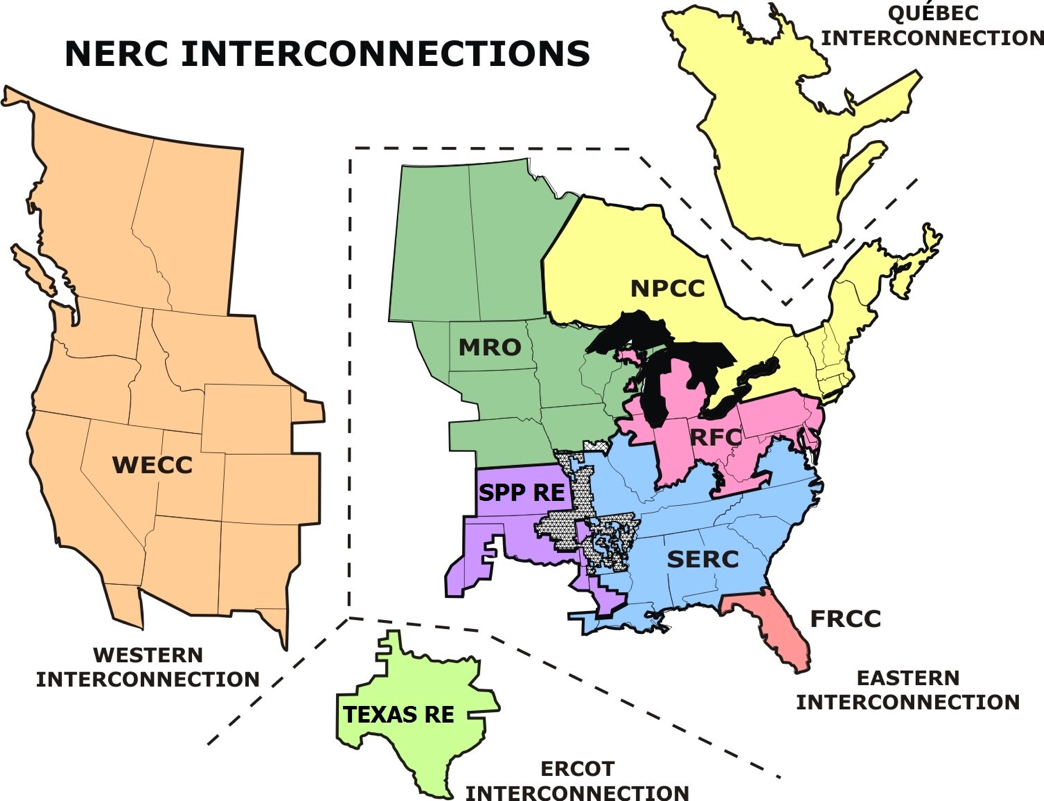
\includegraphics[width=.7\textwidth]{figures/nerc_interconnections}
\caption{The interconnections of North America.  Interconnections have independent frequencies because they are connected with DC lines.  Image from \cite{nerc_image}.}
\label{interconnections}
\end{figure}

Several entities are involved with controlling, regulating, and operating our power systems so they are safe, secure, and reliable for consumers and producers.  In 2005, Congress gave the Federal Energy Regulatory Commission (FERC) the task of overseeing reliability of electric power systems and the power to appoint an organization to perform these tasks~\cite{ferc_215}.  Prior to this, federal involvement in power systems only consisted of price regulation.  In 2006, FERC gave the North America Electric Reliability Corporation (NERC) the authority to regulate the reliability and security of the bulk power system in North America~\cite{nerc}.  All electric utility companies must follow NERC statutes to ensure proper coordination of power flow.  While NERC regulates the entire North American system, it can be broken up into several interconnections where utilities in these interconnections are electrically tied together, as shown in Figure \ref{interconnections}.  These interconnections operate mostly independently of one another.  Within each interconnection exist Independent System Operators (ISO) and Regional Transmission Organizations (RTO).  Both of these entities have similar functions, but RTOs have greater responsibilities outlined by FERC.  ISOs operate their region's grid, oversee the wholesale electricity market, and give reliability planning for the entire region.  RTOs do this and also ensure fair transmission access for utilities \cite{doe_industry_primer}.  Sometimes, ISOs and RTOs can also be the Balancing Authorities (BA) in their region.  BAs are in charge of maintaining the balance between load and generation within their specific areas.  Within each balancing area reside transmission operators, which are in charge of operating their local transmission systems.  Finally, distribution providers control how power flows from transmission operators to end users.

Reliability, stability, and security are key issues for all of these players.  These measures of performance are conducted by each power system entity to determine system risks, upgrades, and instabilities.  The following sections describe these measures, and we pay particular attention to stability, which is most impacted by the addition of renewable generation to the system.

\subsection{Reliability}

Reliability is generally defined as the probability that an item will perform a required function under a specified state~\cite{reliability_def}; a power system's reliability is defined by its ability to maintain an equilibrium between power demand and generation under multiple environmental conditions.  Reliability is the general goal of FERC~\cite{power_reliability}.

A common goal of reliability studies is to determine the likelihood that a component or system will fail.  Depending on modeling goals and assumptions, some cascading failure simulations can provide these type of statistics.  For example, one study found that distributed generation sources in a distribution system can increase the reliability especially during islanding, when a system splits into multiple components, but when these distributed sources come from renewable energy the benefits from the distributed generation can be reduced or even negligible~\cite{dg_reliability}.  Essential modeling techniques in reliability analysis include fault trees, Markov models, and Monte Carlo simulations~\cite{power_reliability}.  Some cascading failure models use probability of failure established by reliability models~\cite{hidden_failures}, whereas some reliability models can use cascading failure models to determine the likelihood of failure~\cite{hines_ig}.  These types of studies are closely related but cascading failure simulations model how blackouts occur whereas reliability analysis quantifies the likelihood of failure under specific conditions.  Reliability is a key concern for power systems, and often, cascading failures occur when various components fail, i.e. become unreliable.

\subsection{Stability}
\label{stability}
Broadly speaking, a power system's stability is its ability to return to an equilibrium state following a disturbance~\cite{kundur}.  The more stable the system is the less likely it will propagate failure.  Although instabilities can \textit{precede} cascading they are more likely to occur \textit{during} a cascade.  For example, an analysis of blackout data shows that most were a result from untrimmed vegetation, followed by failure of protection equipment~\cite{donde}.

There are generally three categories of stability: voltage stability, frequency stability, and rotor angle stability.  First, we introduce voltage stability, which is the system's ability to maintain bus voltages at an acceptable.  Voltage stability depends on the system's ability to restore the equilibrium between load supply and load demand, and the driving force tends to be the loads~\cite{volt_stab}.  One particular type of voltage instability that can lead to cascading failures is Fault-Induced Delayed Voltage Recovery (FIDVR).  This occurs after a fault has been cleared in the system which leads to low voltages.  These low voltages raise the reactive power requirement of motors, particularly air-conditioning units.  When the reactive power cannot be met, the AC units stall, causing them to need 5-6 times the pre-contingency reactive power, this decreases the voltage further and can cause cascading failures~\cite{fidvr_nerc}.  In particular, this can cause voltage collapse, which is when the voltage of the nodes start to drop slowly and then quickly until the system cannot recover.  These scenarios can cause serious damage to equipment and loss of power for a large population if they are not handled properly.

Next, we define frequency stability and rotor angle stability, which are dependent upon generator dynamics.  Frequency stability is when the power system maintains a frequency (50 or 60 Hz) within a specified margin (usually $\pm 0.1$ Hz) after an upset that causes an imbalance between load and generation.  An example of a frequency drop is shown in Figure \ref{fig:frequency}, with relevant terminology labeled.  Large imbalances in load and generation usually occurs due to improper responses of equipment \cite{kundur}.  An example of this occurred in August 2016 when a fire in Southern California caused a fault that exposed improper inverter settings causing unnecessary tripping of equipment for low frequency detection.  This in turn caused the frequency of the system to actually drop, which caused the system to lose 1200 mega-watts of PV power~\cite{nerc_inv}.  
\begin{figure}
\begin{center}
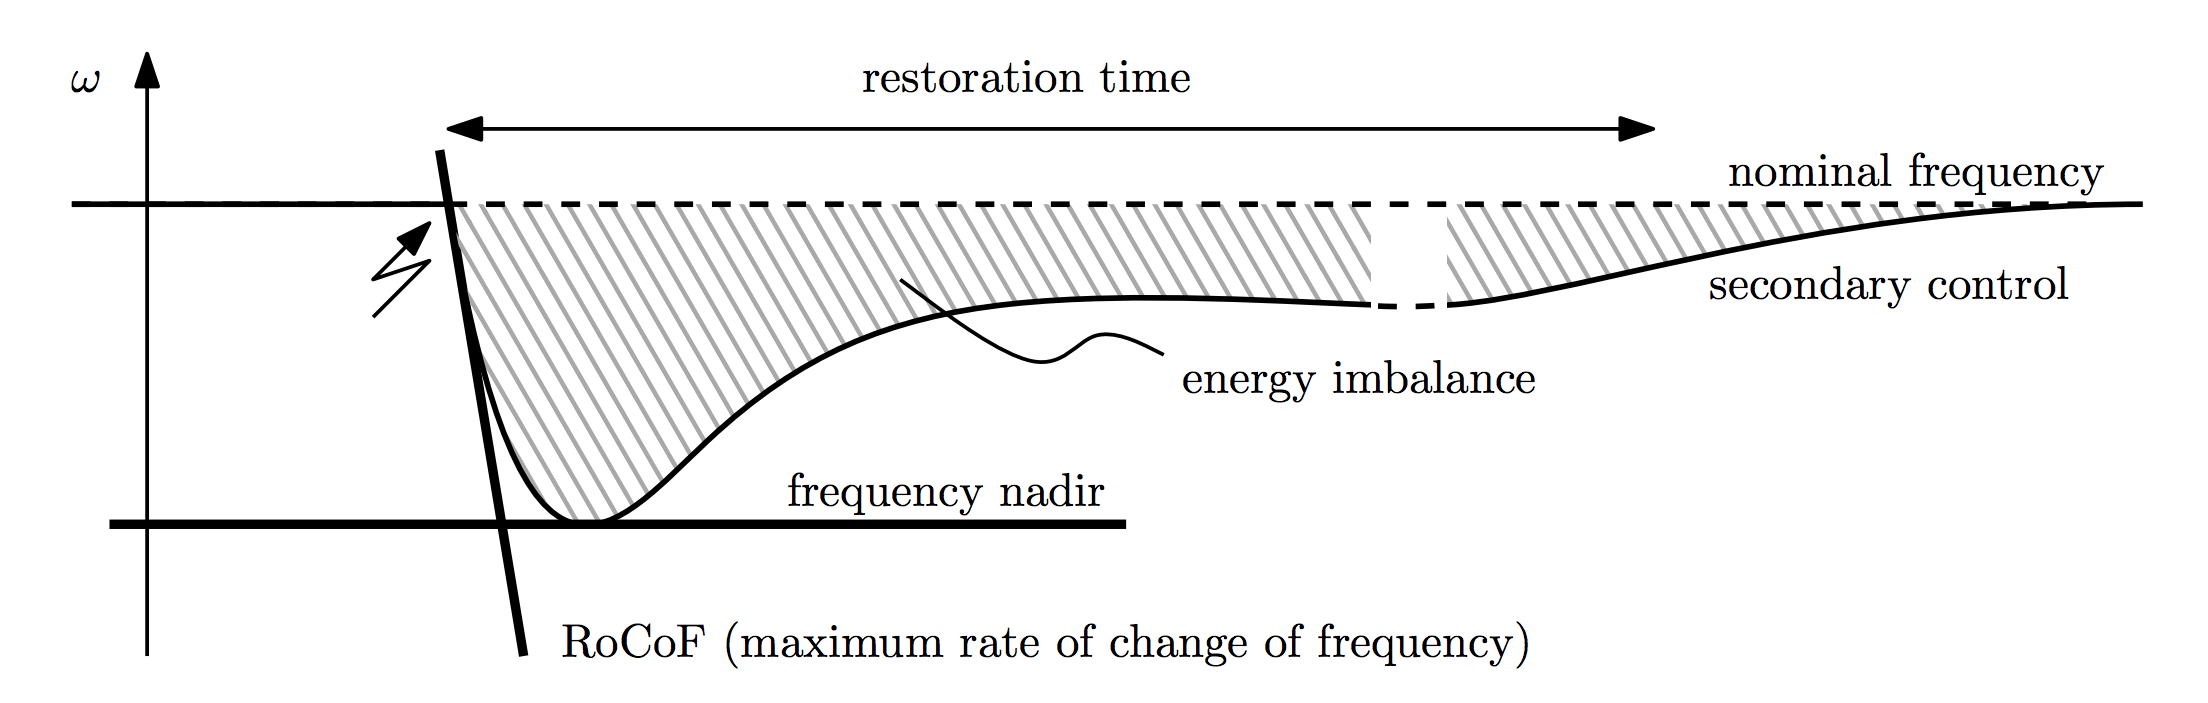
\includegraphics[width=\textwidth]{figures/frequency}	
\caption{An example of a frequency drop. Figure from \cite{Gross}.}
\label{fig:frequency}
\end{center}
\end{figure}
The frequency of a system is generally referred to as the center of inertia, and is computed based on the rotor speeds and inertia constants of the generators in the system \cite{dorfler_inertia}.  This is defined by Equation \ref{eqtn:wcoi}
\begin{equation}
\label{eqtn:wcoi}
\omega_{COI} = \frac{\sum\limits_{g=1}^{n_g} M_g \omega_g}{	\sum\limits_{g=1}^{n_g} M_g}
\end{equation}


However, in practice, system frequency is usually measured at some relevant bus in the system.  This is a less accurate measure of system frequency as it is influenced by generators that are closer to the bus, rather than the average frequency of the whole system.  Thus, the center of inertia frequency is largely used in simulations.    Closely related to frequency stability is rotor angle stability, which refers to a generator's oscillations.  When a generator becomes out of sync with other generators due to an instability, usually rebalancing forces from other generators restore it to the proper oscillation speed and phase.  This is dependent on the system's ability to restore the equilibrium between the mechanical and electromagnetic torque of the generator.  The system becomes unstable when it cannot absorb the kinetic energy caused from the differences in rotor speeds~\cite{def_stability}.  

Frequency stability and rotor angle stability have become a prominent research area the past decade due to the increase in renewable generation sources.  
	

The study of power system instabilities is concerned with identifying the system's \textit{response to} instability.  Instabilities are usually involved with cascading failures (such as hidden failures of protection equipment) but may not be the primary cause.  Some cascading failure models use various instabilities as a reason for line tripping, thus furthering a cascade, but because of the complexity required, very few employ these dynamics explicitly.  Modeling the instabilities themselves is generally thought of as separate from modeling cascading failures because of the level of detail (i.e. ACPFE, DAE) required for instability analysis.


\subsection{Security}
A power system's ability to handle instabilities partly determines its robustness, but two systems that are equally stable might not be equally secure as one could have more severe consequences from a failure~\cite{security_def}.  NERC requirements determine how secure a power system must be under various types of operating conditions. A canonical regulation requires all transmission systems to be $n-1$ secure which means if any one component fails, power can still flow to all loads~\cite{nerc_stand}.  However, there are less security requirements for $n-k$ contingencies because they are numerous and it is hard to determine which sets of these contingencies have higher risk and should be prevented.  Overall, a power system's security measures its ability to maintain reliability and stability due to a specified perturbation.


Reliability, stability, and security analyses have suggested improvements for increasing the resiliency of power systems.  But, cascading failures are still inevitable despite our best efforts to avoid them.  Understanding how failure propagates through an electrical system and what factors increase the likelihood and size of the blackout is the concern of cascading failure modeling.  In the next section, we will review various cascading failure models which highlight various properties of power systems and determine why blackouts are inevitable in modern power systems.






   



























